% Dies ist Teil der Vorlesung Physik auf dem Computer, SS 2012,
% Axel Arnold, Universitaet Stuttgart.
% 
% Dieses Werk ist unter einer Creative Commons-Lizenz vom Typ
% Namensnennung-Weitergabe unter gleichen Bedingungen 3.0 Deutschland
% zugänglich. Um eine Kopie dieser Lizenz einzusehen, konsultieren Sie
% http://creativecommons.org/licenses/by-sa/3.0/de/ oder wenden Sie sich
% schriftlich an Creative Commons, 444 Castro Street, Suite 900, Mountain
% View, California, 94041, USA.

\chapter{Lineare Gleichungssysteme \textrm{II}}
\index{Gleichungssysteme>lineare}

\begin{figure}
  \centering
  \begin{tikzpicture}[node distance=0em and 0em]
    \node (pic) {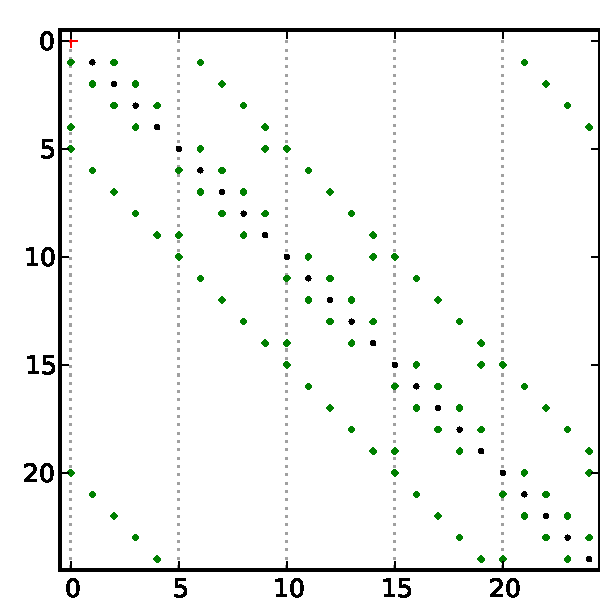
\includegraphics[height=9\baselineskip]{plots/2d-laplace}};
    \node[right= of pic] {
      $\cdot\begin{pmatrix}
        \Phi_0 = \phi(0,0)\\
        \Phi_1 = \phi(h,0)\\
        \vdots\\
        \Phi_{4} = \phi(h,0)\\
        \Phi_{5} = \phi(0,h)\\
        \vdots\\
        \Phi_{24} = \phi(4h,4h)
      \end{pmatrix}
      =-
      \begin{pmatrix}
        \Phi_0\\
        \rho(h,0)\\
        \vdots\\
        \rho(h,0)\\
        \rho(0,h)\\
        \vdots\\
        \rho(4h,4h)
      \end{pmatrix}
      $ } ;
  \end{tikzpicture}
  \caption{Symbolische Darstellung der Gleichung zum Laplace-Operator
    in zwei Dimensionen, diskretisiert auf einem $5\times
    5$-Gitter. In der Matrix markieren grüne Punkte Einträge mit Wert
    $1/h^2$, schwarze mit $-4/h^2$ und das rote Kreuz den
    Normierungseintrag mit Wert 1. Alle anderen Einträge sind
    Null. Die ersten fünf Elemente einer Matrixzeile numerieren
    jeweils zunächst die Gitterpunkte $(k h, 0)$, $k=0(1)4$,
    durch. Die folgenden fünf Elemente der Matrixzeile entsprechen $(k
    h, h)$, und so weiter. Durch die periodischen Randbedingungen sind
    auch sehr weit entfernte Nebendiagonalen teilweise besetzt.}
  \label{fig:2d-laplace}
\end{figure}

Wie wir bereits gesehen haben, lassen sich gewöhnliche
Differentialgleichungen in einer Dimension recht einfach auf lineare
Gleichungssysteme abbilden. Diese haben Bandstruktur und sind
effizient zu lösen.  In mehr als einer Dimension ist das allerdings im
allgemeinen nicht mehr der Fall. Betrachten wir zum Beispiel die
Poissongleichung in zwei Dimensionen:
\begin{equation}
  \label{eq:laplace}
  \Delta \phi = \frac{\partial^2 \phi}{\partial x^2} +
  \frac{\partial^2 \phi}{\partial y^2} = \rho.
\end{equation}
Wir diskretisieren nun wie gewohnt $\phi(x,y)$ in beiden Dimensionen
zu $\phi_{k, l} = \phi(k h, l h)$, $k,l=(1)N$. Den Laplace-Operator
erhalten wir dann in erster Ordnung als
\begin{align}
  \label{eq:laplacedisc}
  \Delta \phi(k h, l h) \approx
  \frac{1}{h^2}\bigl(\phi_{k+1,l} -
  2\phi_{k,l}  + \phi_{k-1,l}\bigr) + 
  \frac{1}{h^2}\bigl(\phi_{k,l+1} -
  2\phi_{k,l}  + \phi_{k,l-1}\bigr)\nonumber\\
  = \frac{1}{h^2}\bigl(
  \phi_{k,l+1} + \phi_{k+1,l} - 4\phi_{k,l} +
  \phi_{k-1,l} + \phi_{k,l-1}\bigr).
\end{align}
Der Einfachheit halber nehmen wir periodische Randbedingungen an, so
dass wir diese Gleichung für jeden Gitterpunkt aufstellen
können. Allerdings wäre die resultierende Matrix singulär; um die
Differenzialgleichung mit periodischen Randbedingungen eindeutig lösen
zu können, müssen wir einen Funktionswert vorgeben.

Diese Gleichungen sind im Moment noch auf der Matrix $\phi_{k,l}$
definiert, die wir nun \emph{linearisieren} müssen, um die Gleichung
in der gewohnten Matrixform etwa an Python zu übergeben. Hierzu
speichern wir die Elemente von $\phi_{k,l}$ wie folgt:
\begin{equation}
  \Phi_{k + N l} = \phi_{k,l} \quad\text{für}\; k,l=1(1)N.
\end{equation}
Wie man sich leicht überlegt, ist diese Zuordnung eindeutig, wir
können also beliebig zwischen $\Phi_n$ und $\phi_{k,l}$ wechseln und
so etwa \eqref{eq:laplacedisc} auf den Vektor $\Phi_n$
übertragen. Dies ergibt dann $N^2$ Gleichungen für alle Datenpunkte,
die in Matrixform wie Abbildung~\ref{fig:2d-laplace} aussehen.

Abbildung~\ref{fig:2d-laplace} zeigt, dass die entstehende Matrix zwar
immer noch Bandstruktur hat und dünn besetzt ist, d.h. fast alle
Einträge Null, allerdings sind diese Bänder nicht mehr nur um die
Diagonale verteilt. Auch durch Umsortieren lässt sich dies nicht
wesentlich verbessern. Daher muss die volle Gaußelimination
durchgeführt werden. Für Gitter von $5\times 5$ Punkten ist das zwar
noch ausreichend schnell zu lösen, bei einem Gitter von $100\times
100$ Punkten hat die Matrix allerdings bereits $100,000,000$ Einträge,
was die Gaußelimination ziemlich langsam macht.

Im folgenden lernen wir nun schnellere, iterative Gleichungslöser
kennen, mit denen auch solche und größere Gleichungssysteme handhabbar
werden. Außerdem lernen wir Verfahren zur Berechnung von Eigenwerten
und -vektoren kennen und eine wichtige Verallgemeinerung, die
Singulärwertzerlegung. Diese leitet dann schon wieder zum nächsten
Kapitel, der Optimierung, über.

\section{Iterative Gleichungslöser}

Wir betrachten eine reguläre Matrix $A\in\RR^{n,n}$ und einen Vektor
$b\in\RR^n$. Gesucht ist dann die Lösung $\overline{x}\in\RR^n$ mit
\begin{equation}
  \label{eq:axb}
  A\overline{x} = b.
\end{equation}

Die Gaußelimination liefert diese bei unendlicher Genauigkeit exakt,
allerdings mit dem hohen Aufwand $\O(n^3)$. Wir haben allerdings
bereits gesehen, dass iterative Verfahren wie etwa das Newtonverfahren
zur Lösung nichtlinearer Gleichungssysteme quadratisch
konvergieren. Daher suchen wir ein iteratives Verfahren der Form
\begin{equation}
  \label{eq:itgl}
  x^{(i+1)} = G(x^{(i)}) = T x_i + r
\end{equation}
mit $r\in\RR^n$ und $T\in\RR^{n,n}$, $\norm{T}<1$, damit die
sukzessive Substitution für jeden Startwert konvergiert, wobei die
Norm $\norm{\cdot}$ wiederum geeignet gewählt werden kann.

Wie müssen wir nun $T$ wählen, damit einerseits $x^{(i)}\to \overline{x}$
für $i\to\infty$, andererseits aber $T$ und $r$ einfach zu berechnen
sind? Da $\norm{T} < 1$ sein soll, muss $r$ bereits eine
Näherungslösung sein. Es sollte also $r = B^{-1}b$ sein, wobei $B$
eine geeignete, einfach zu invertierende Näherung von $A$ ist. Dann
gilt
\begin{equation}
  \overline{x} = T\,\overline{x} +
  B^{-1}b
  \stackrel{!}{=} T\,\overline{x} +
  B^{-1}A\,\overline{x}
  = \left(T + B^{-1}A\right)\overline{x},
\end{equation}
was sich offenbar durch Wahl von $T = I - B^{-1}A$ erfüllen
lässt. Solange also $B^{-1}$ einfach zu bestimmen ist, lassen sich
sowohl $T$ als auch $r$ einfach berechnen.

\subsection{\keyword{Jacobiverfahren}}

Beim Jacobiverfahren wird die Matrix also Summe einer Diagonalmatrix
sowie einer linken, unteren
und einer rechten oberen Dreiecksmatrix mit verschwindender Diagonale
zerlegt, also $A = L + D + U$ mit
\begin{equation}
  l_{ik}=
  \begin{cases}
    a_{ik} & \text{für}\; i<k\\
    0 & \text{sonst}
  \end{cases},\quad
  d_{ik} =
  \begin{cases}
    a_{ik} & \text{für}\; i=k\\
    0 & \text{sonst}
  \end{cases}\quad\text{und}\;
  u_{ik} =
  \begin{cases}
    a_{ik} & \text{für}\; i>k\\
    0 & \text{sonst}
  \end{cases}.
\end{equation}
Die Diagonalmatrix $D$ soll dabei die Rolle der leicht zu
invertierenden Matrix übernehmen. Dazu müssen die Diagonalelemente
alle von Null verschieden sein, wass sich bei einer regulären Matrix
$A$ durch Vertauschen von Zeilen und/oder Spalten immer erreichen
lässt.

Setzen wir also $T=I-D^{-1}A$ und $r=D^{-1}b$ in \eqref{eq:itgl} ein,
so erhalten wir das \emph{Jacobiverfahren}
\begin{align}
  x^{(i+1)} = \left(I - D^{-1}A\right)x^{(i)} + D^{-1}b\nonumber\\
  = -D^{-1}\left(L + U\right)x^{(i)} + D^{-1}b
\end{align}
mit der Diagonalmatrix $D$, so dass $d^{-1}_{jj} =
\frac{1}{a_{jj}}$. Komponentenweise bedeutet dies, dass
\begin{equation}
  \label{eq:jacobicomp}
  x_j^{(i+1)} = \frac{1}{a_{jj}}\left(b_j - \sum_{k\neq j} a_{jk}x_k^{(i)}\right).
\end{equation}
Mit anderen Worten, dass Jacobiverfahren löst jede Zeile nach der
Variablen auf der Diagonale auf.

\index{strikt diagonaldominant}
Wann konvergiert dieses Verfahren? Eine gängige Voraussetzung ist,
dass die Matrix $A$ strikt diagonaldominant ist, also
\begin{equation}
  \sum_{k\neq i} \abs{a_{ik}} < \abs{a_{ii}}\quad\text{für}\; i=1(1)n.
\end{equation}
Diese Bedingung wird zum Beispiel von der Matrix aus dem
Eingangsbeispiel erfüllt.  Matrizen, die durch Diskretisierung von
Differentialgleichungen entstehen, sind sogar meist von dieser Form.

Ist $A$ strikt diagonaldominant, so nutzen wir die Maximumsnorm
\begin{equation}
  \norm{A}_\infty := \max_{i=1}^n \sum_{k=1}^n \abs{a_{ik}},
\end{equation}
die eine Matrixnorm definiert. Dann gilt
\begin{equation}
  \norm{T}_{\infty} = \norm{I-D^{-1}A}_{\infty} =
  \max_{i=1}^n \sum_{k\neq i} \frac{\abs{a_{ik}}}{\abs{a_{ii}}} < 1,
\end{equation}
die sukzessive Substitution und damit das Jacobiverfahren konvergieren
also. Außerdem ist die Konvergenz linear, genauer gilt
\begin{equation}
  \frac{\norm{x_{n+1} - \overline{x}}_\infty}{\norm{x_{n} - \overline{x}}_\infty}
  \le \sum_{k\neq i} \frac{\abs{a_{ik}}}{\abs{a_{ii}}},
\end{equation}
wobei $\norm{x}_\infty := \max_{i=1}^n \abs{x_i}$ die
Vektormaximumsnorm bezeichnet. Je größer also die Diagonaleinträge
gegenüber den Nebeneinträgen sind, desto schneller konvergiert das
Verfahren, zum Beispiel wenn die Matrix eine kleine Störung der
Einheitsmatrix ist.

\subsection{\keyword{Gauß-Seidel-Verfahren}}

Wird \eqref{eq:jacobicomp} zeilenweise abgearbeitet, so müssen die
bereits bearbeiteten Werte $x_k^{(i+1)}$ zwischengespeichert werden,
da für die restlichen Zeilen ja noch die alten Werte $x_k^{(i+1)}$
benötigt werden. Beim Gauß-Seidel-Verfahren werden stattdessen die
bereits berechneten, neueren Werte benutzt:
\begin{equation}
  x_j^{(i+1)} = \frac{1}{a_{jj}}\left(b_j -
    \sum_{k=1}^{j-1} a_{jk}x_k^{(i+1)} - \sum_{k=j+1}^n a_{jk}x_k^{(i)}\right).
\end{equation}
Mit der Zerlegung $A=L + D + U$ wie
beim Jacobiverfahren ergibt sich in Matrixschreibweise
\begin{equation}
  x^{(i+1)} = -D^{-1}L x^{(i+1)} - D^{-1} U x^{(i)} + D^{-1}b
  \;\implies\;
  (D + L)x^{(i+1)} = - U x^{(i)} + b
\end{equation}
und damit
\begin{equation}
  x^{(i+1)} = -(D+L)^{-1} U x^{(i)} - (D+L)^{-1}b.
\end{equation}
Das Gauß-Seidel-Verfahren ist also auch vom Typ \eqref{eq:itgl}, mit
der etwas komplexeren Matrix $B= (D+L)^{-1}$. Tatsächlich ist auch
\begin{equation}
  T = I - (D + L)^{-1} A = (D + L)^{-1}(D + L - A) = -(D+L)^{-1} U.
\end{equation}
Man kann zeigen, dass $\norm{T}_\infty$ beim Gauß-Seidel-Verfahren
kleiner ist als beim Jacobi-Verfahren. Das bedeutet allerdings im
allgemeinen nicht, dass das Gauß-Seidel-Verfahren schneller ist. Man
spart allerdings den Speicherplatz, um $x^{(i+1)}$
zwischenzuspeichern.

Insbesondere für die parallele Verarbeitung, die mit der heutigen
weiten Verbreitung von Mehrkern-Prozessoren immer wichtiger ist, ist
das Gauß-Seidel-Verfahren allerdings ungeeignet, da die Berechnung
jeder Zeile die Ergebnisse der vorherigen erfordert. Das
Jacobi-Verfahren kann hingegen auf soviele Prozessoren verteilt
werden, wie die Matrix Zeilen hat, was eine effiziente Verarbeitung
selbst auf modernen Graphikkarten ermöglicht. 

\subsection{\keyword{Relaxationsverfahren}}
\index{Successive Overrelaxation}
\index{SOR}

Beim Relaxationsverfahren (Successive Over-relaxation, SOR) wird statt
$B = D + L$ die Matrix $B = D/\omega + L$ mit einem geeigneten
Relaxationsfaktor $\omega$ betrachtet. Durch geeignete Wahl von
$\omega$ können dann auch nicht strikt diagonaldominante Matrizen
behandelt werden. Allerdings kann man nur zeigen, dass $0<\omega< 2$
gelten muss, aber ein Wert $\omega$, der zu schneller Konvergenz
führt, muss durch Ausprobieren gefunden werden.

In Matrixschreibweise gilt analog
\begin{equation}
  T = I - \omega(D + \omega L)^{-1} A = (D +
  \omega L)^{-1}(D + \omega L - \omega A) = -(D+\omega L)^{-1}
  \left[\omega U + (\omega-1) D\right]
\end{equation}
und damit
\begin{equation}
  x^{(i+1)} = -(D+\omega L)^{-1}
  \left[\omega U + (\omega-1) D\right]x^{(i)} +
  \omega(D + \omega L)^{-1} b
\end{equation}
beziehungsweise
\begin{equation}
  x^{(i+1)} = -\omega D^{-1}L x^{(i+1)}
  -\left[\omega D^{-1}U + (\omega-1)I\right]x^{(i)} +
  \omega D^{-1}b.
\end{equation}
In Komponentenschreibweise schließlich ergibt sich
\begin{equation}
  x_j^{(i+1)} = \frac{\omega}{a_{jj}}\left(
    b_j
    - \sum_{k=1}^{j-1} a_{jk} x_k^{(i+1)}
    - \sum_{k=j+1}^{n} a_{jk} x_k^{(i)}\right)
  + (1-\omega) x_j^{(i)}.
\end{equation}
$\omega$ gewichtet also zwischen der Beibehaltung der vorherigen
Näherung und dem der nächsten Gauß-Seidel-Iterierten. Insofern ist es
erstaunlich, dass auch Werte $\omega>1$ sinnvoll sein können, die die
bestehende Näherungen quasi bestrafen.

%%% Local Variables: 
%%% mode: latex
%%% TeX-master: "padc.tex"
%%% TeX-PDF-mode: t
%%% End: 
